\section{Sistemi Operativi per smartphone: \\ Android e iOS}
L'applicazione è stata realizzata tramite il framework Flutter (a cui sarà
dedicato l'intero prossimo capitolo), in modo tale da poter sviluppare lo stesso
progetto per i due maggiori sistemi operativi per smartphone, Android di
proprietà di Google e iOS dell'azienda Apple. In questo capitolo si prendono in
considerazione tali sistemi focalizzandosi soprattutto sul funzionamento.

\subsection{Android}
Android è un sistema operativo mobile, realizzato per dispositivi mobili
touchscreen, ed è stato sviluppato inizialmente dall'azienda Android Inc., che
nel 2005 è stata acquistata da Google. [inserisci fonte] \\
Una delle caratteristiche più importanti di questo sistema operativo è che
detiene una licenza open source. Questo tipo di licenza consente liberamente a
qualsiasi utente di modificare e distribuire liberamente il codice
sorgente, consentendo quindi una continua evoluzione del sistema operativo e una
più semplice diffusione. Considerando i processi, Android riesce a gestirli in
modo da mantenere il consumo energetico al minimo. Quando un’applicazione non è
in uso, il sistema sospende il suo funzionamento ma allo stesso tempo la rende
disponibile per l’uso immediato, così che l’applicazione non contribuisca
al consumo della batteria. Il sistema operativo gestisce le applicazioni archiviate in
memoria, in modo tale che sull'esaurirsi della memoria volatile il sistema inizi
automaticamente a chiudere i processi, partendo da quelli che sono rimasti
inattivi per il periodo di tempo più lungo.

\subsubsection{Kernel Linux e Architettura}
Un kernel può essere considerato come un ponte tra hardware e software, e può comunicare con
l’hardware tramite i driver che sono inclusi al suo interno. In questo modo, quando
un’applicazione vuole rispondere a un comando, può inoltrare le istruzioni al
kernel e quest’ultimo può utilizzare i driver dell’hardware che vogliamo
controllare per ottenere il comportamento desiderato. In particolare, Android si
appoggia al kernel Linux (fig. \ref{kernel}). Esso fornisce
tutte le funzioni essenziali per il sistema, tra cui: la gestione della memoria
primaria e la gestione delle risorse hardware del sistema e delle periferiche.
Il suo incarico quindi è quello di gestire
il tempo processore, le comunicazioni e la memoria, assegnando ogni cosa ai processi in
corso in base alle priorità assegnate. Il kernel Linux è adatto a tutte quelle
tecnologie embedded più rilevanti, e quindi ha avuto molto successo nel campo
delle tecnologie portatili.
Esso è inoltre utilizzato dal sistema operativo Android, sebbene Google abbia
introdotto qualche variazione. Una di queste è la funzionalità di gestione
del risparmio, chiamata “wakelocks”, che impedisce al telefono di lavorare a
basso consumo. Nel kernel Linux non c’è un’implementazione completa della
Libreria Standard del linguaggio C++ (STL), dato che le applicazioni Android si
basano sul linguaggio di programmazione Java, dunque ciò che è scritto in codice
C/C++ deve essere richiamato da codice java. Questo porta al fatto che tutte le chiamate a
sistema fatte in C/C++ devono chiamare la Java Virtual Machine. Oltre al
kernel Linux, Android è formato anche da  middleware, Librerie e API scritte in C/C++. Le
ultime versioni di Android usano ART Virtual Machine, mentre nelle vecchie versioni
veniva utilizzata la Dalvik Virtual Machine (entrambe considerate nel prossimo
paragrafo).
\begin{figure}
    \centering
    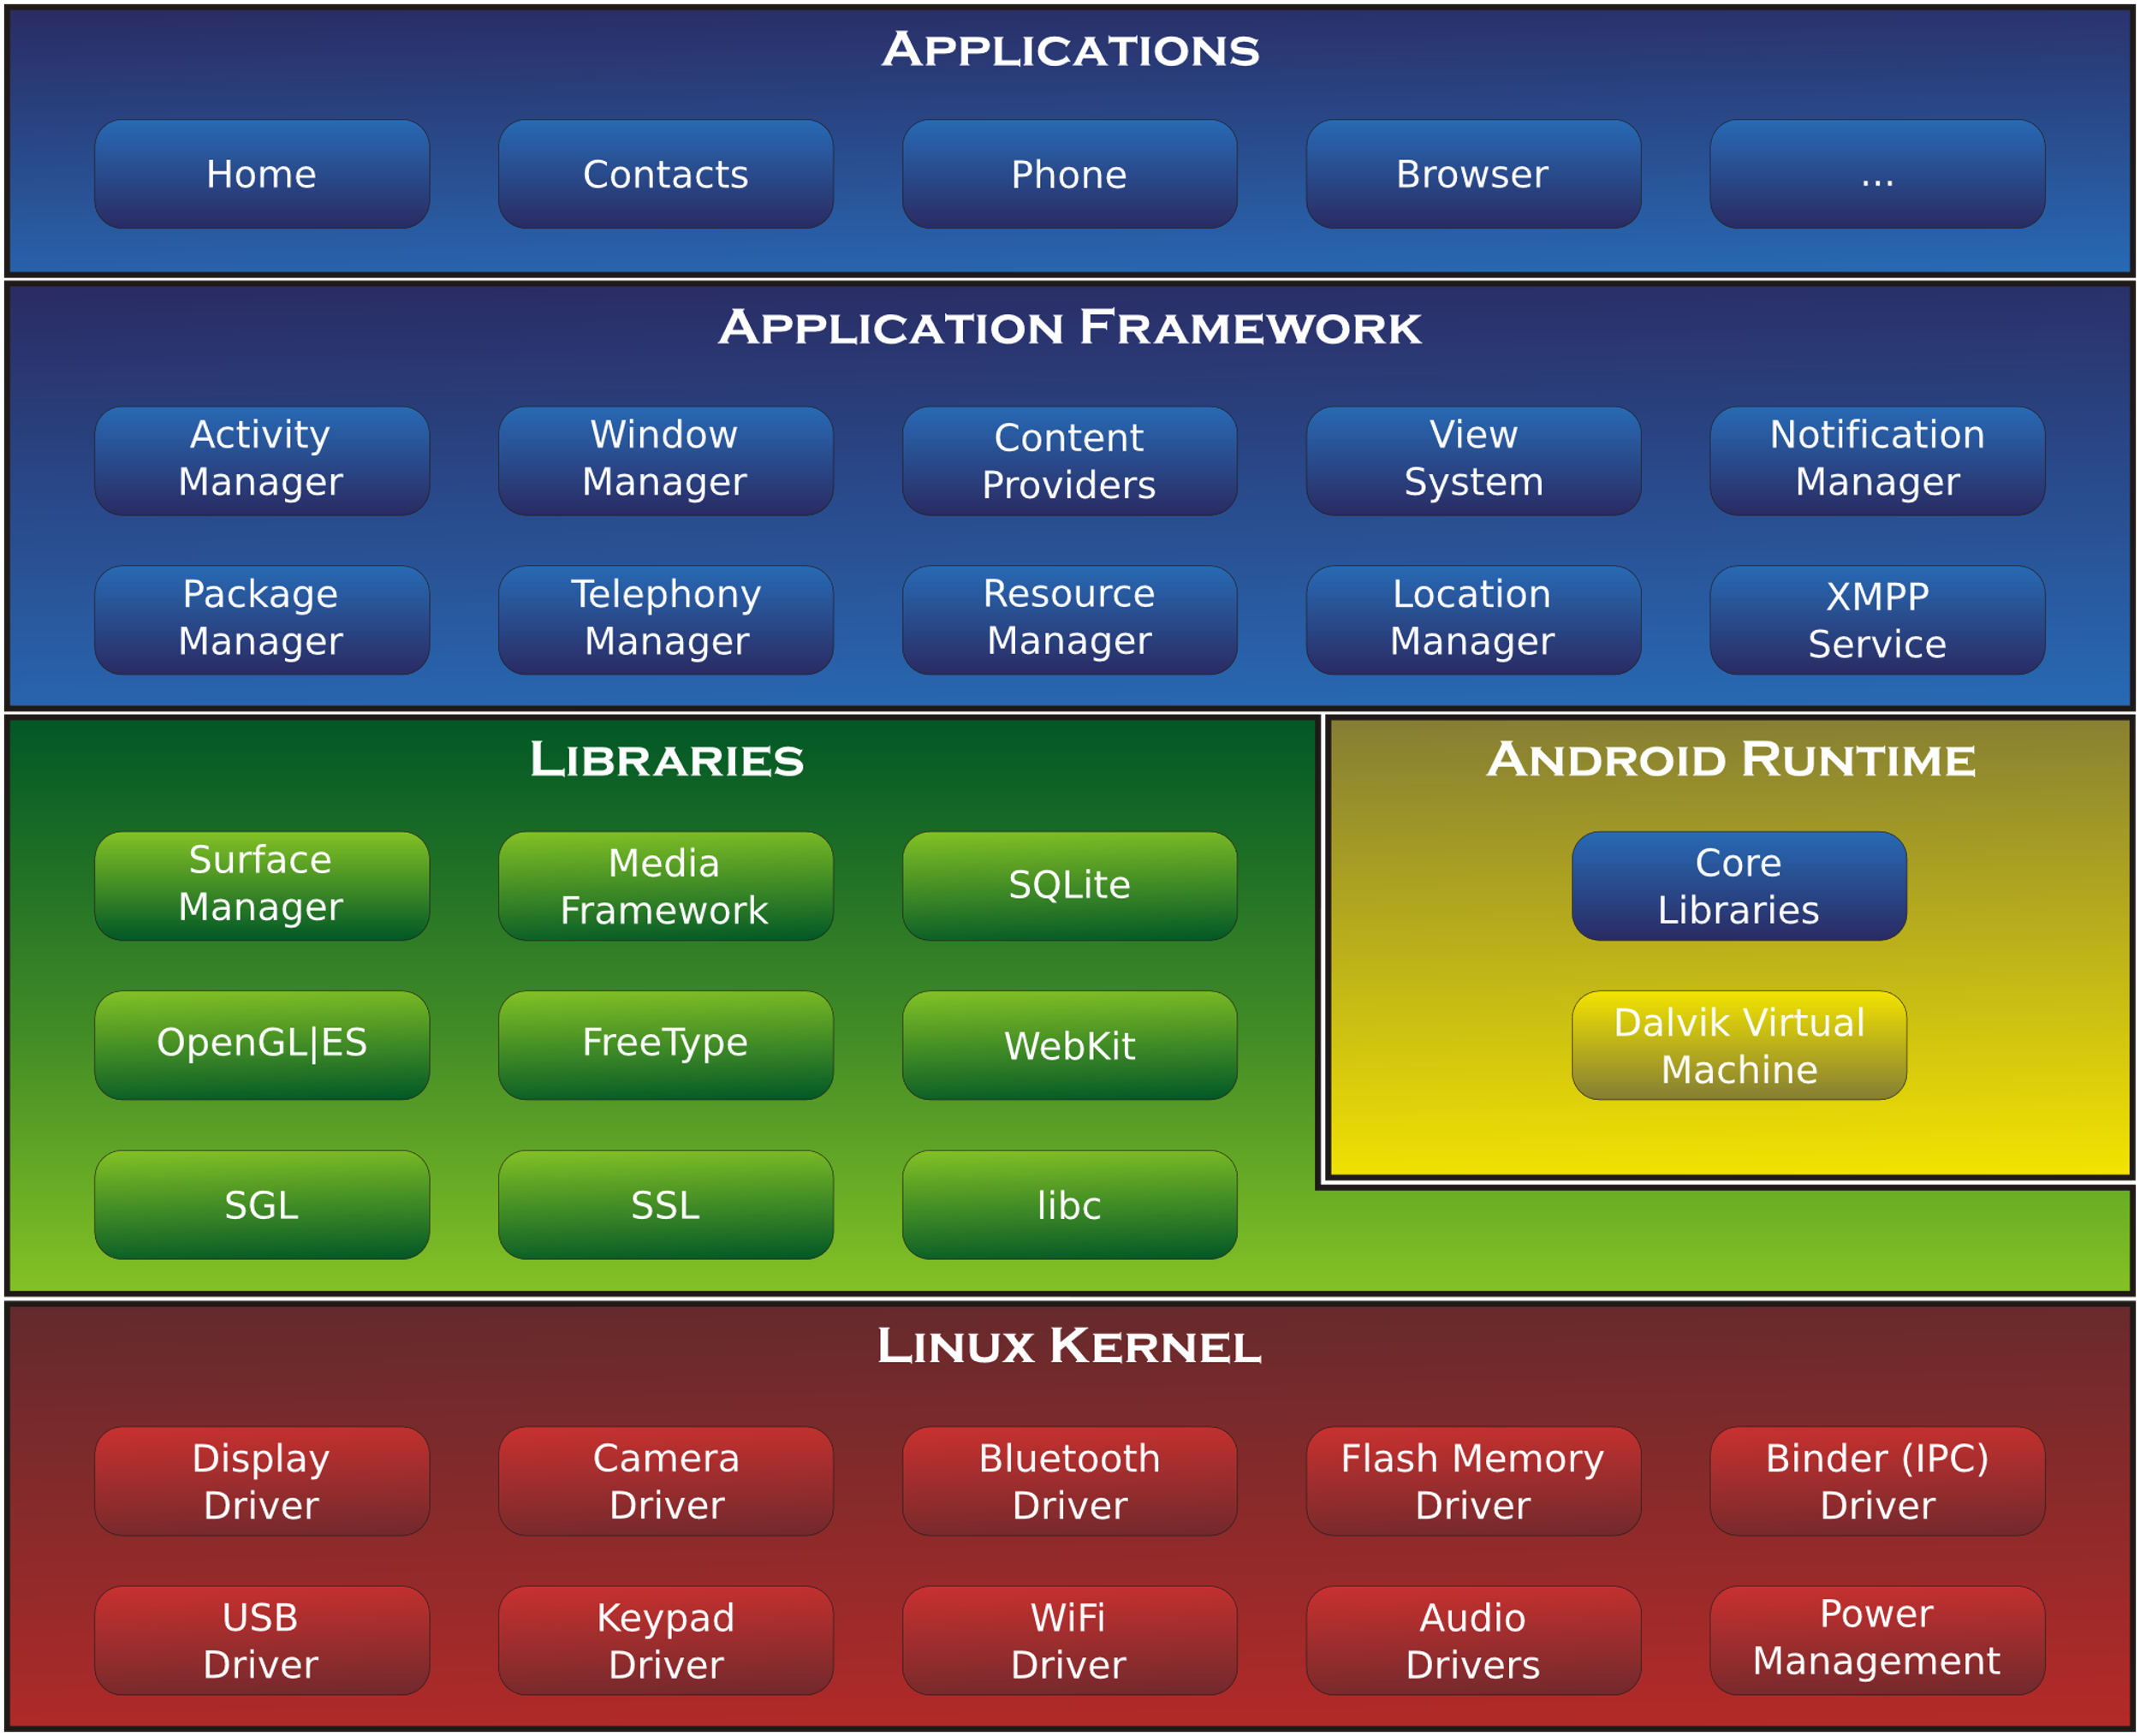
\includegraphics[width=9.5cm]{kernel.png}
    \caption{Struttura del sistema operativo Android e del kernel Linux}
    \label{kernel}
\end{figure}

\subsubsection{ART Virtual Machine e Dalvik Virtual Machine}
La VM, Virtual Machine, è in Android il software all’interno del
quale vengono eseguite le applicazioni. Le applicazioni Android vengono scritte in
linguaggio Java, il quale viene poi compilato in Bytecode
(intermedio tra il linguaggio macchina e il linguaggio di
programmazione che permette che il codice possa essere eseguito su macchine
diverse con hardware diversi), compilato infine
dalla Virtual Machine. Inizialmente in Android veniva utilizzata la Dalvik VM,
che a partire dalla versione 4.4 KitKat di Android, è stata sostituita dalla ART
VM.
La VM Dalvik è basata su tecnologia \textit{just-in-time}: ogni applicazione viene
compilata solo in parte dal programmatore e sarà poi di volta in volta dovere
della Dalvik VM eseguire il codice e compilarlo in linguaggio macchina in tempo
reale. Questo ovviamente grava sulle prestazioni.
La ART VM invece è basata su tecnologia \textit{ahead-of-time} che esegue l'intera
compilazione del codice durante l'installazione dell'applicazione e non durante
l'esecuzione stessa del software. Questo permette di avere un vantaggio in
termine di prestazioni, anche se incide sul tempo di installazione delle
applicazioni.

\subsubsection{Sviluppo applicazioni in Android}
In aiuto ai programmatori per la scrittura di applicazioni Android esiste un
kit di sviluppo software  chiamato SDK. L’SDK  comprende un numeroso set di
strumenti di sviluppo, tra cui: librerie software, debugger, documentazione e
codice d’esempio. Esistono poi diversi ambienti per lo sviluppo, tra questi si
ricordano Visual Studio Code, Atom, Eclipse e Android Studio. Quest'ultimo è considerato l'IDE
primario per lo sviluppo di applicazioni, in quanto presenta notevoli agevolazioni.
I progetti Android sono costituiti da parti dinamiche scritte in Java e
parti statiche scritte in XML. L’SDK permette  di eseguire le applicazioni sia
in emulazione, sia su un dispositivo vero e proprio. Per descrivere
l’applicazione allo smartphone che si vuole utilizzare, si fa ricorso al file
Manifest.xml, questo elenca la lista delle necessità del software per poter
funzionare in modo adeguato. Per motivi di sicurezza, per evitare che
applicazioni di terze parti abbiano i permessi per poter accedere a informazioni
private all’interno del
telefono, bisogna controllare attentamente il contenuto del Manifest, e non
installare il software in caso richieda risorse non coerenti con lo scopo
dichiarato dell’applicazione. Una volta scritta e concluso il progetto, il
codice java e il codice XML vengono compilati generando un file con estensione
.apk (l’eseguibile delle applicazioni Android). Esso contiene il bytecode che verrà
mandato eseguito dalla Virtual Machine. Le applicazioni Android sono pilotate
dagli eventi (Event Driven), cioè azioni che vengono causate da hardware o da altri
componenti. Il programmatore quindi sviluppa per ogni hardware routine
indipendenti, permettendo al sistema operativo di rinunciare al caricamento di
componenti che non si andranno a utilizzare, e utilizzando solo quelli che sono
strettamente necessari. \\
Quando si avvia per la prima volta un dispositivo Android, si può notare come su
tale sistema siano già presenti
applicazioni di terze parti, che possono essere utilizzate fin da subito
dagli utenti. Quando si vuole utlizzare un'applicazione non ancora presente sul
proprio smartphone bisogna scaricare e installare il file apk dell’applicazione
dal Google Play Store. Quest’ultimo è il principale "negozio" di
applicazioni installato su dispositivi Android, e consente agli utenti di
scaricare e aggiornare le applicazioni pubblicate da Google o sviluppatori di
terze parti. Esistono infine anche un certo numero di mercati di app di terze
parti, che forniscono servizi che non possono essere offerti dallo store
ufficiale a causa di violazioni di particolari norme.

